\documentclass[10.5pt,a4paper]{article}
\usepackage[utf8]{inputenc}
\usepackage[T1]{fontenc}
\usepackage[catalan]{babel}
\usepackage{lmodern,microtype}
\usepackage[margin=2cm,top=1.8cm,bottom=1.8cm]{geometry}
\usepackage{amsmath,amssymb,graphicx,booktabs,float,caption,subcaption,hyperref,enumitem,array,tikz}
\usepackage{listings,xcolor}
\usetikzlibrary{arrows.meta,positioning}
\hypersetup{colorlinks=true,linkcolor=blue!50!black,citecolor=blue!50!black,urlcolor=blue!50!black}
\captionsetup{font=small,labelfont=bf}
\setlist{itemsep=1pt,topsep=2pt,parsep=0pt}
\setlength{\parskip}{3pt}
\lstset{basicstyle=\ttfamily\scriptsize,breaklines=true,frame=single,backgroundcolor=\color{gray!8},columns=fullflexible,keepspaces=true,language=Python}
\newcommand{\py}[1]{\texttt{\detokenize{#1}}}

\title{\vspace{-1.3cm}\textbf{Classificació i detecció d'anomalies en un catàleg sísmic global amb $K$-Means i distància als $k$ veïns}}
\author{Matias Stein Niell}
\date{}

\begin{document}
\maketitle
\vspace{-1.2cm}
\begin{abstract}
\noindent Aquest informe presenta un sistema en Python (pandas + scikit-learn) que agrupa $10\,174$ esdeveniments sísmics d'arreu del món (USGS, 15/09--15/10/2026) amb $K$-Means i detecta els més atípics amb la distància mitjana als $k$ veïns més propers. Es descriuen les decisions de disseny, cada part del codi i els resultats, validats amb silueta, índex de Davies--Bouldin, estabilitat entre llavors (ARI), sensibilitat a $k$ i contrast amb Isolation Forest i LOF. Els tres clústers ($5\,721$/$3\,414$/$1\,039$; silueta $0{,}402$) reflecteixen sobretot \emph{l'abast geogràfic de cada xarxa sísmica} (Califòrnia, Alaska, món) i no una tipologia tectònica; la partició és totalment estable (ARI $=1$). Les 5 anomalies són terratrèmols profunds (286--665~km) en zones de subducció, i no els més grans.
\end{abstract}

%------------------------------------------------------------
\section{Plantejament del problema}
\subsection{Context i interès}
Els serveis sismològics registren milers d'esdeveniments al mes, la gran majoria de magnitud petita; revisar-los un a un és inviable. Calen procediments automàtics que (a) els organitzin en grups amb propietats semblants, (b) assenyalin els casos excepcionals que mereixen l'atenció d'un sismòleg i (c) ajudin a detectar si un grup reflecteix la física del terratrèmol o simplement com es mesura (cobertura de les xarxes). El problema connecta amb el tòpic de l'exposició, l'\emph{aprenentatge no supervisat} (clustering i detecció d'anomalies): no hi ha etiquetes ``correctes'', de manera que la qualitat s'ha de provar amb criteris interns i contrastos entre mètodes.

\subsection{Objectius mesurables}
\begin{description}[leftmargin=1.1cm,labelwidth=0.9cm]
\item[O1] Carregar i netejar el catàleg conservant el $100\,\%$ de les files amb magnitud, profunditat, latitud i longitud vàlides.
\item[O2] Particionar els esdeveniments en $K=3$ grups, caracteritzar-los (mida, magnitud, profunditat, regió) i assolir una silueta mitjana $\bar s>0{,}3$ (estructura moderada \cite{kaufman}).
\item[O3] Identificar els 5 esdeveniments més anòmals i interpretar-ne l'origen.
\item[O4] Avaluar l'estabilitat del clustering respecte a la llavor aleatòria (objectiu: ARI $\ge0{,}95$) i el cost computacional (objectiu: $<1$~s per fase).
\item[O5] Contrastar l'elecció de $K$ i la llista d'anomalies amb alternatives (altres $K$, altres $k$, Isolation Forest, LOF).
\end{description}

\subsection{Abast i supòsits}
S'usa un únic fitxer (\py{earthquakes.csv}, format USGS ComCat \cite{usgs}) i quatre variables numèriques: magnitud, profunditat (km), latitud i longitud. \emph{Supòsits:} (i) la distància euclidiana sobre variables estandarditzades és una mesura de semblança admissible; (ii) $K=3$ és fix i es contrasta a posteriori; (iii) latitud i longitud es tracten com a variables lineals tot i que la longitud és circular (discutit a la Secció~\ref{sec:lim}). \emph{Fora d'abast:} predicció sísmica, mecanisme focal i estimació de risc.

%------------------------------------------------------------
\section{Fonamentaci\'o te\`orica}
\subsection{Les dades s\'ismiques}
Un esdeveniment s'identifica per la seva localitzaci\'o (latitud, longitud, profunditat de l'hipocentre) i la seva magnitud, una mesura logar\'itmica de l'energia alliberada. La magnitud de moment $M_w$ \cite{hanks} \'es la m\'es consistent f\'isicament, per\`o els catàlegs barregen escales (\py{ml}, \py{md}, \py{mb}, \py{mww}\ldots) segons la xarxa i la mida de l'esdeveniment; en aquest fitxer predominen \py{ml} (6\,668), \py{md} (2\,468) i \py{mb} (889). La distribuci\'o de magnituds segueix aproximadament la llei de Gutenberg--Richter \cite{gr}, $\log_{10}N=a-bM$: hi ha moltes magnituds baixes i molt poques d'altes, la qual cosa condiciona tant el clustering com la detecci\'o d'anomalies.

\subsection{Normalitzaci\'o $z$-score}
Com que la profunditat (0--665 km) t\'e una escala molt superior a la magnitud ($-1{,}3$--$7{,}7$), una dist\`ancia sense escalar estaria dominada per la profunditat. Cada variable $j$ es transforma en
\begin{equation}
z_{ij}=\frac{x_{ij}-\mu_j}{\sigma_j},\qquad \mu_j=\frac1n\sum_i x_{ij},\quad \sigma_j=\sqrt{\frac1n\sum_i (x_{ij}-\mu_j)^2},
\end{equation}
de manera que totes tenen mitjana 0 i desviaci\'o 1. Si $\sigma_j=0$ es fixa $\sigma_j=1$ per evitar una divisi\'o per zero.

\subsection{K-Means (algorisme de Lloyd)}
K-Means \cite{lloyd,macqueen} cerca $K$ centroides $\mathbf c_1,\dots,\mathbf c_K$ que minimitzen la inercia
\begin{equation}
J=\sum_{i=1}^{n}\min_{k}\,\lVert \mathbf z_i-\mathbf c_k\rVert^2 ,
\end{equation}
iterant dues passes: assignaci\'o de cada punt al centroide m\'es proper i actualitzaci\'o de cada centroide com a mitjana del seu grup. Cada iteraci\'o costa $O(nKd)$, per\`o nom\'es garanteix un m\'inim local, per la qual cosa el resultat depn\'en de la inicialitzaci\'o (existeix \py{k-means++} \cite{kmpp} per millorar-la). Com a alternatives: DBSCAN (no requereix $K$ i detecta soroll, per\`o exigeix triar $\varepsilon$ i densitat), models de mixtura gaussiana (cl\'usters el\textperiodcentered l\'iptics i assignaci\'o suau) i el cl\'uster jer\`arquic ($O(n^2)$ en mem\`oria).

\subsection{Detecci\'o d'anomalies per dist\`ancia als $k$ ve\"ins}
Es defineix la puntuaci\'o d'anomalia d'un punt com la mitjana de les dist\`ancies als seus $k$ ve\"ins m\'es propers \cite{ramaswamy}:
\begin{equation}
s(\mathbf z)=\frac1k\sum_{m=1}^{k} d\bigl(\mathbf z,\mathbf z_{(m)}\bigr).
\end{equation}
Els punts en regions poc denses tenen $s$ alt. \'Es una t\`ecnica simple i interpretable, per\`o $O(n^2)$ i sensible a $k$ i a l'escala. Alternatives: LOF (compara densitats locals), Isolation Forest i m\`etodes de reconstrucci\'o \cite{chandola}.

\subsection{M\`etriques de validaci\'o}
El \emph{coeficient de silueta} \cite{rousseeuw} d'un punt \'es $s_i=(b_i-a_i)/\max(a_i,b_i)$, on $a_i$ \'es la dist\`ancia mitjana al seu cl\'uster i $b_i$ la dist\`ancia mitjana al cl\'uster alternatiu m\'es proper; val entre $-1$ i $1$. L'\emph{\'index de Rand} compara dues particions parella a parella (1 = id\`entiques) i s'usa per mesurar l'estabilitat entre llavors.

%------------------------------------------------------------
\section{Metodologia i solució proposada}
\subsection{Visió general i estructura del codi}
La solució consta de només dos scripts (Figura~\ref{fig:pipe}). \py{presentacio_MATIAS.py} conté les funcions del projecte (càrrega, normalització, $K$-Means, anomalies i gràfic), cadascuna amb una única responsabilitat, docstring i paràmetres en lloc de valors fixos, i el pipeline principal que les encadena. \py{validacio_MATIAS.py} \emph{importa} aquestes funcions i hi afegeix l'avaluació de $K$ i de l'estabilitat, l'anàlisi complementària (Isolation Forest, LOF, sensibilitat a $k$), els gràfics de validació i les proves automàtiques; així la lògica (primer fitxer) queda separada de la validació i les proves (segon fitxer). S'usen \py{pandas} \cite{pandas}, \py{scikit-learn} \cite{sklearn} i \py{matplotlib} \cite{mpl} en lloc d'implementacions pròpies, per fiabilitat i velocitat.

\begin{figure}[H]
\centering
\begin{tikzpicture}[node distance=0.35cm,every node/.style={draw,rounded corners,font=\scriptsize,align=center,minimum height=0.9cm,fill=blue!6}]
\node (a) {CSV\\\py{read_csv}};
\node (b) [right=of a] {Neteja\\\py{dropna}};
\node (c) [right=of b] {$z$-score\\(4 variables)};
\node (d) [right=of c] {$K$-Means\\$K=3$};
\node (e) [right=of d] {kNN ($k=5$)\\puntuació $s$};
\node (f) [right=of e] {Top-5 +\\gràfics};
\foreach \x/\y in {a/b,b/c,c/d,d/e,e/f}{\draw[-{Latex[length=1.5mm]}] (\x)--(\y);}
\end{tikzpicture}
\caption{Fases de \py{presentacio_MATIAS.py}, cada una implementada per una funció del mateix fitxer. \py{validacio_MATIAS.py} reutilitza les fases 1--3 i afegeix l'avaluació de $K$, l'estabilitat i el mapa.}\label{fig:pipe}
\end{figure}

\subsection{Parts del codi, funcions i justificació}
\begin{table}[H]
\centering\footnotesize
\begin{tabular}{@{}>{\raggedright\arraybackslash}p{3.7cm}>{\raggedright\arraybackslash}p{12.9cm}@{}}
\toprule
\textbf{Funció} & \textbf{Paper i justificació}\\
\midrule
\py{carrega_dades(path)} & \py{pd.read_csv} i \py{dropna(subset=features)}: elimina només les files amb NaN a les 4 variables usades. Comprova que hi ha les columnes i que queda alguna fila (\py{ValueError}); \py{FileNotFoundError} si el fitxer no existeix.\\
\py{normalitza_zscore(df)} & $z$-score vectoritzat per columnes (\py{(X-X.mean())/X.std()}); si una columna és constant, fixa $\sigma=1$ per evitar divisions per zero. Preferit a min--max perquè els extrems (profunditat $>600$~km, $M>7$) comprimirien la resta.\\
\py{entrena_kmeans(X,k)} & \py{KMeans(random_state=42, n_init=10)}: \py{k-means++} amb 10 reinicis i es queda la menor inèrcia (evita mínims locals). Valida que $1\le k\le n$.\\
\py{resum_clusters(df)} & \py{groupby("cluster").agg}: nombre, magnitud i profunditat mitjanes per clúster.\\
\py{puntuacio_anomalia(X,k)} & \py{NearestNeighbors(n_neighbors=k+1).kneighbors}: distàncies exactes; se n'ignora la columna 0 (el propi punt) i es fa la mitjana dels $k$ restants $\Rightarrow$ puntuació $s$. \py{top_anomalies} tria les $n$ més altes amb \py{nlargest}.\\
\py{avalua_k}, \py{avalua_estabilitat} (a \py{validacio_MATIAS.py}) & Inèrcia, \py{silhouette_score} (mostra de 2\,000 punts i dades senceres) i \py{davies_bouldin_score} per a cada $K$; \py{adjusted_rand_score} entre la llavor 42 i les llavors 1--5.\\
\py{contrast_detectors}, \py{sensibilitat_k}, \py{experiment_mag_prof} (a \py{validacio_MATIAS.py}) & Isolation Forest i LOF de \py{scikit-learn} amb correlació de Spearman; coincidència del top-5 en variar $k$; $K$-Means només amb magnitud i profunditat.\\
\py{figura_clusters}, \py{figura_mapa}, \py{figura_k}, \py{figura_anomalies} & Només dibuixen (\py{scatter}, eix de profunditat invertit perquè creix cap avall, anomalies com a quadrats vermells) i desen el PNG; no calculen res.\\
\bottomrule
\end{tabular}
\caption{Elements del codi i la seva funció.}\label{tab:funcs}
\end{table}

El nucli de la detecció d'anomalies és breu i exacte (sense mostreig):
\begin{lstlisting}
def puntuacio_anomalia(X, k_veins=5):
    if not 1 <= k_veins < len(X):                       # validacio d'entrada
        raise ValueError(...)
    veins = NearestNeighbors(n_neighbors=k_veins + 1).fit(X)   # +1: el primer vei es ell mateix
    distancies, _ = veins.kneighbors(X)
    return distancies[:, 1:].mean(axis=1)               # puntuacio d'anomalia s
\end{lstlisting}

\subsection{Decisions de disseny justificades}
\textbf{$K=3$}: hipòtesi de tres règims (petit i superficial, intermedi, gran i profund); contrastada amb $K=2,\dots,8$ (Taula~\ref{tab:k}). \textbf{Distància exacta als veïns} (no mostrejada): amb $n\approx10^4$ costa $<0{,}1$~s, per tant no cal aproximar. \textbf{$k=5$}: valor petit que detecta regions molt buides; se'n comprova la sensibilitat (Secció~\ref{sec:anom}). \textbf{Mateixa normalització} a ambdós scripts perquè els resultats siguin comparables.

%------------------------------------------------------------
\subsection{Proves automàtiques}
\py{validacio_MATIAS.py} conté \textbf{35 proves} (\py{unittest}, també detectades per \py{pytest}) que s'executen automàticament abans de la validació en $\approx1$~s i passen totes: \emph{casos normals} (el $z$-score deixa mitjana 0 i desviació 1; $K$-Means separa tres grups sintètics ben definits; l'outlier obvi obté la puntuació més alta; la puntuació val exactament $1{,}5$ en un exemple calculat a mà); \emph{casos límit} (columna constant, punts duplicats, $K=1$, \py{sample_size} superior a $n$, NaN en columnes no usades, demanar més anomalies de les que hi ha); \emph{casos erronis} (fitxer inexistent, columna que falta, tot NaN, $k$ no vàlid, $K$ fora de rang); la generació de les figures; i una \emph{prova d'integració} que comprova que amb \py{earthquakes.csv} es reprodueixen els resultats d'aquest informe (10\,174 files, mides $5\,721/3\,414/1\,039$, inèrcia $19\,486{,}7$, primera anomalia i profunditats $>280$~km); també es proven les funcions de l'anàlisi complementària.

%------------------------------------------------------------
\section{Resultats i anàlisi}\label{sec:res}
\subsection{Neteja i descripció de les dades}
Les $10\,174$ files són vàlides (cap NaN a les 4 variables; O1 complert). Magnitud: $-1{,}29$ a $7{,}70$ (mitjana $1{,}71$); profunditat: $-3{,}4$ a $665$~km (mitjana $22{,}9$, mediana $8{,}1$; $351$ valors negatius per elevació del terreny); data entre 15/09 i 15/10/2026. Hi ha $9\,938$ terratrèmols i $236$ esdeveniments d'altres tipus que el programa \textbf{no filtra} ($132$ voladures de pedrera, $73$ explosions, $27$ \emph{ice quakes}, $4$ altres). Xarxes dominants: \py{ak} (2\,446), \py{nc} (1\,538), \py{ci} (1\,326), \py{us} (1\,215), \py{tx} (837), \py{av} (798). Les escales de magnitud es barregen (\py{ml} 6\,668, \py{md} 2\,468, \py{mb} 889, \py{mww} 102).

\subsection{Clústers trobats}
\begin{table}[H]
\centering\footnotesize
\begin{tabular}{@{}crrrrrrl@{}}
\toprule
Clúster & $n$ & $\bar M$ & $\bar p$ (km) & $p_{max}$ & $\bar\varphi$ & $\bar\lambda$ & Xarxes dominants\\
\midrule
0 & 3\,414 & 1,52 & 33,0 & 243,6 & 58,9 & $-154{,}8$ & \py{ak} (2\,425), \py{av} (781): Alaska\\
1 & 5\,721 & 1,31 & 7,7 & 88,2 & 33,8 & $-114{,}4$ & \py{nc}, \py{ci}, \py{tx}, \py{hv}: Califòrnia, Texas, Hawaii\\
2 & 1\,039 & 4,50 & 73,0 & 665,1 & 5,9 & 49,4 & \py{us} (985): global, $M\gtrsim4$\\
\bottomrule
\end{tabular}
\caption{Perfil dels clústers ($K=3$). $\bar M$: magnitud mitjana; $\bar p$, $p_{max}$: profunditat mitjana i màxima; $\bar\varphi,\bar\lambda$: centre geogràfic.}\label{tab:cl}
\end{table}

\begin{figure}[H]
\centering
\begin{subfigure}[t]{0.49\textwidth}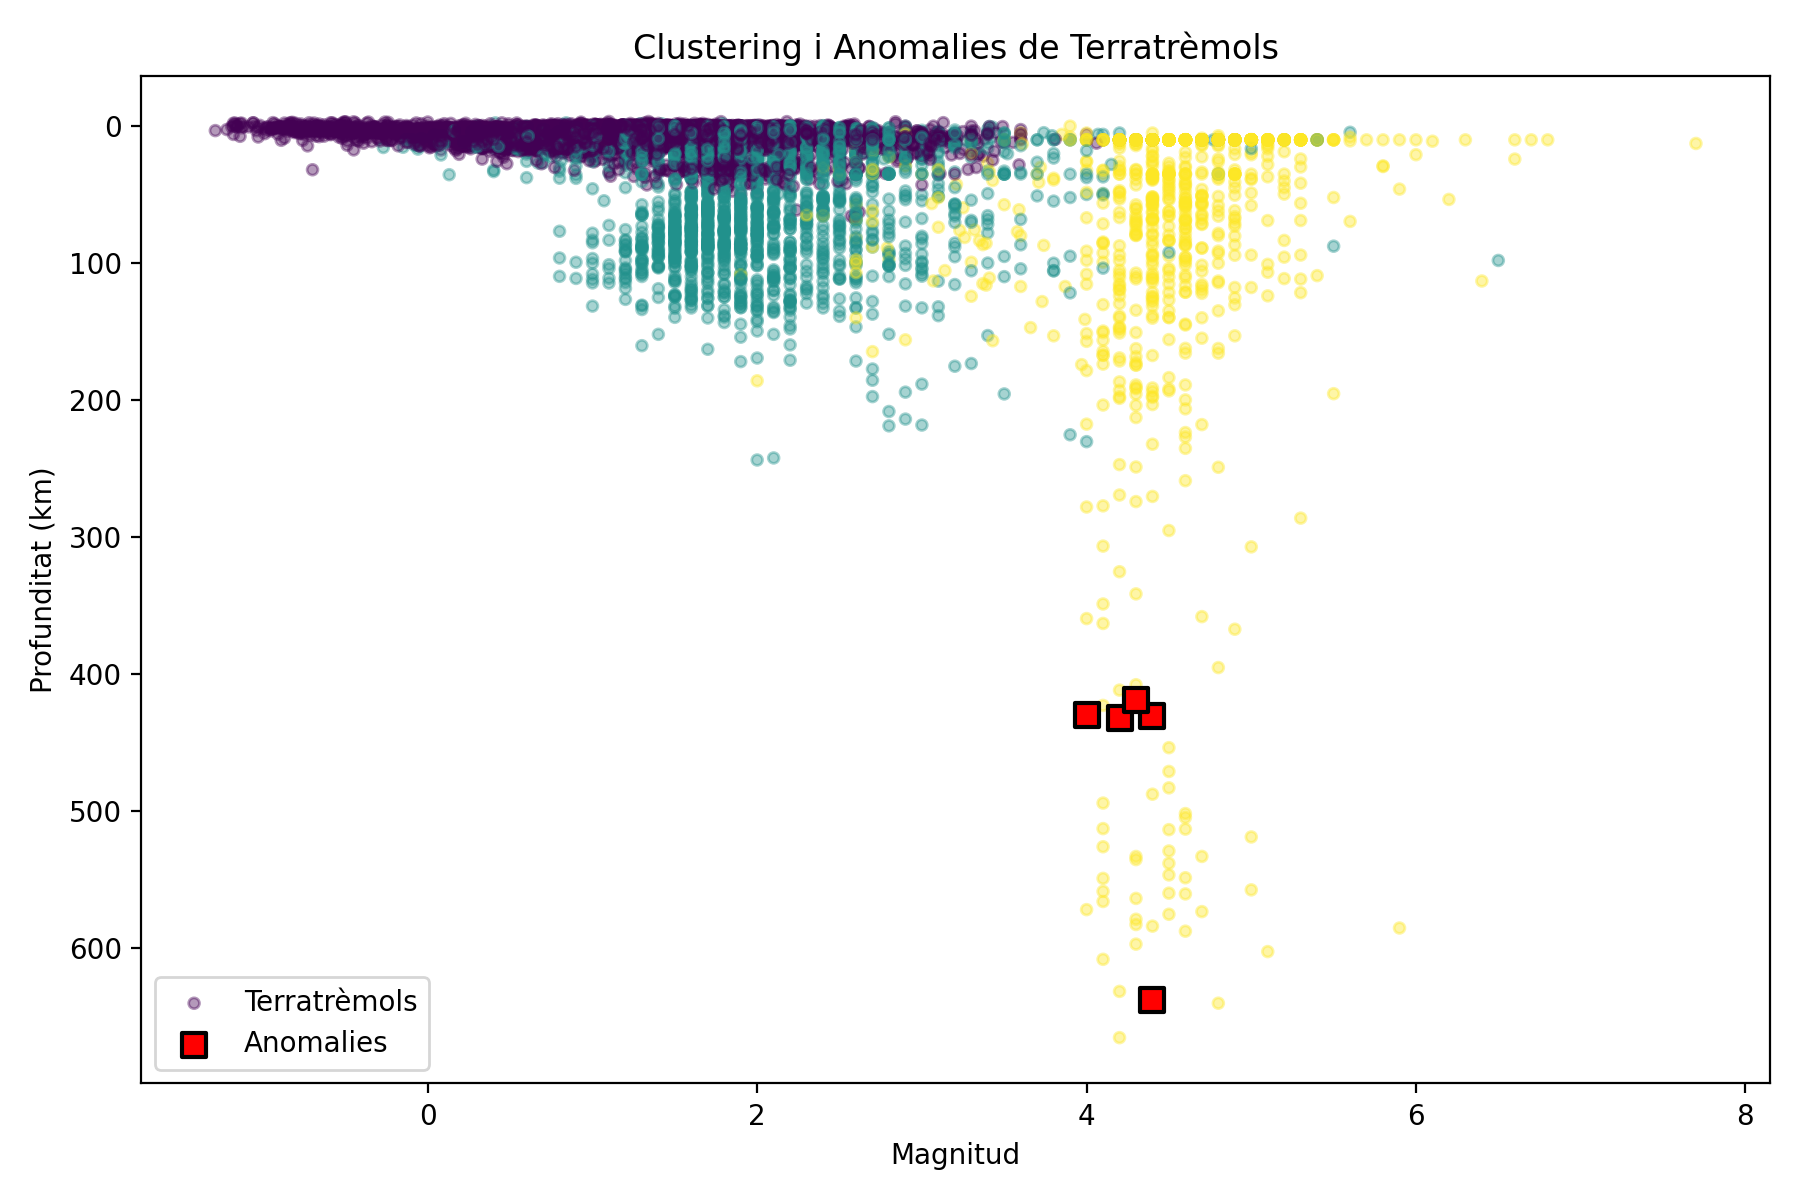
\includegraphics[width=\linewidth]{fig_clusters.png}\caption{Magnitud vs.\ profunditat (eix invertit).}\end{subfigure}\hfill
\begin{subfigure}[t]{0.49\textwidth}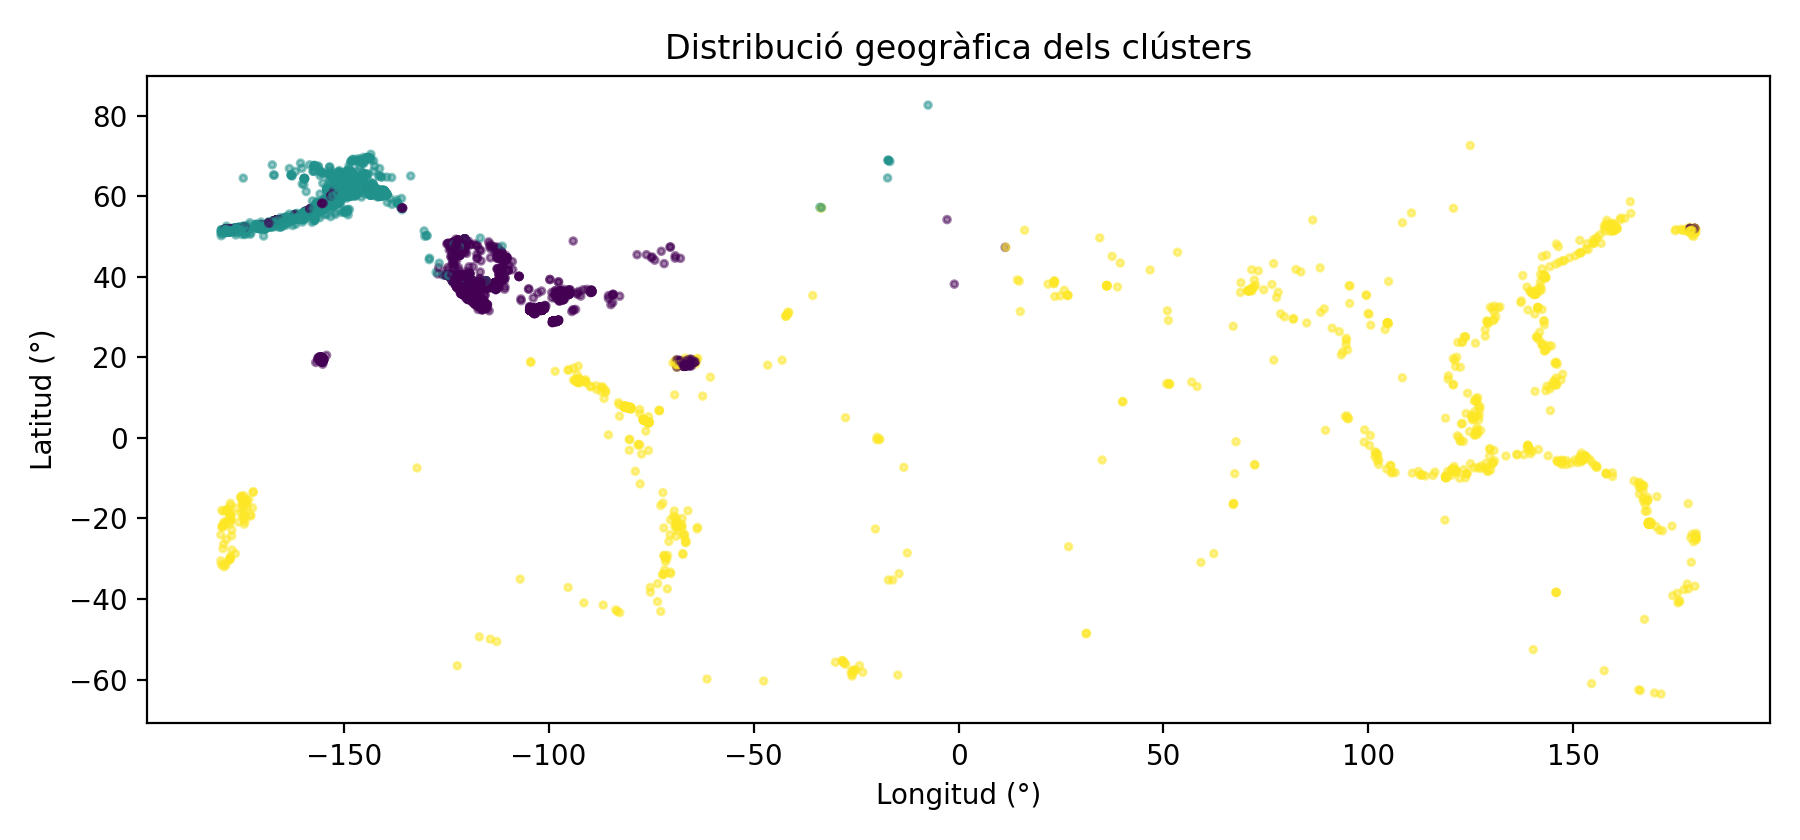
\includegraphics[width=\linewidth]{fig_mapa.png}\caption{Distribució geogràfica.}\end{subfigure}
\caption{Clústers de $K$-Means (mateixos colors a ambdós panells: lila = 0, verd = 1, groc = 2). A (a), els quadrats vermells són les 5 anomalies.}\label{fig:cl}
\end{figure}

\textbf{Interpretació crítica.} El clúster~1 agrupa esdeveniments petits i superficials de xarxes regionals de Califòrnia, Texas i Hawaii; el~0, esdeveniments petits i de profunditat moderada a Alaska (zona de subducció, xarxa molt sensible); el~2, la sismicitat global registrada per l'USGS, que només inclou $M\gtrsim4$ (magnitud mínima $1{,}27$, mitjana $4{,}50$). El mapa (Fig.~\ref{fig:cl}b) mostra que \textbf{els clústers se separen per regió}: latitud i longitud, dues de les quatre variables, tenen molta variació i dominen la distància. El clúster~2 és ``gran'' sobretot per \emph{cobertura del catàleg} (una xarxa regional detecta $M<1$, la global no), no per la física. Un indici addicional de la limitació de tractar la longitud com a lineal: els esdeveniments de les Aleutianes a $\lambda\approx+179^\circ$ cauen al clúster~2 (groc) tot i ser veïns dels de $\lambda\approx-179^\circ$ (lila).

\subsection{Validació: elecció de $K$ i qualitat}
\begin{table}[H]
\centering\footnotesize
\begin{tabular}{@{}lrrrrrrr@{}}
\toprule
$K$ & 2 & 3 & 4 & 5 & 6 & 7 & 8\\
\midrule
Inèrcia $J$ & 24\,346 & 19\,487 & 14\,659 & 12\,256 & 10\,184 & 8\,780 & 7\,623\\
Silueta (mostra 2\,000) & 0,640 & 0,411 & 0,417 & 0,427 & 0,334 & 0,358 & 0,358\\
Silueta (totes les dades) & 0,654 & 0,402 & 0,414 & 0,422 & 0,338 & 0,360 & 0,360\\
Davies--Bouldin & 0,925 & 1,042 & 0,905 & 0,989 & 0,948 & 0,906 & 0,884\\
\bottomrule
\end{tabular}
\caption{Inèrcia i índexs de qualitat per a $K=2,\dots,8$ (llavor 42, \py{n_init=10}).}\label{tab:k}
\end{table}
\begin{figure}[H]
\centering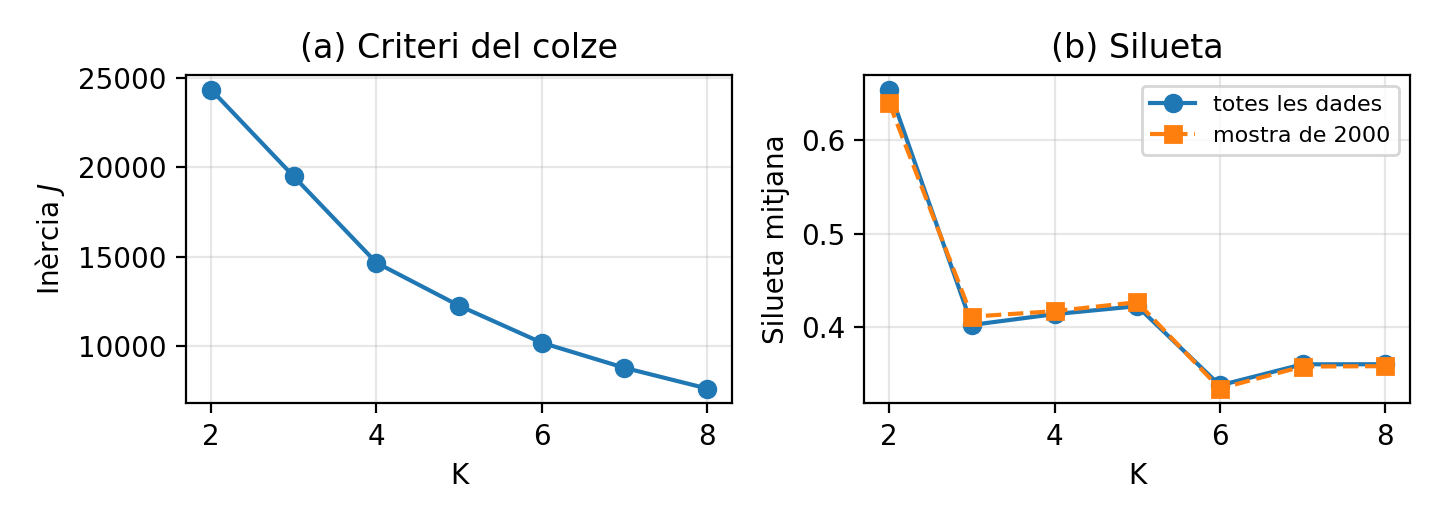
\includegraphics[width=0.72\textwidth]{fig_k.png}
\caption{(a) Inèrcia en funció de $K$: no hi ha un colze clar. (b) Silueta mitjana: el màxim és a $K=2$.}\label{fig:k}
\end{figure}
Amb $K=3$ la silueta és $0{,}402$ (totes les dades; la mostra de $2\,000$ en dona $0{,}411$, diferència de $0{,}009$, per tant el mostreig és fiable): O2 complert. Per clúster és molt desigual: $0{,}530$ (clúster~1, compacte), $0{,}256$ (clúster~0) i només $0{,}177$ (clúster~2, molt heterogeni: cobreix tot el planeta). \textbf{$K=2$ obté la millor silueta ($0{,}654$)}, i en aquest cas separa essencialment el clúster global ($1\,039+18$ esdeveniments) de tota la resta regional (matriu de contingència: $3\,413+5\,704$ regionals queden junts). La corba d'inèrcia no té colze i Davies--Bouldin no afavoreix cap $K$ de manera clara. Per tant $K=3$ és una elecció defensable per interpretabilitat (separa Alaska de Califòrnia), però \emph{no és òptima segons les mètriques}.

\textbf{Estabilitat.} Amb les llavors $1$--$5$, l'ARI respecte a la llavor 42 és $1{,}0000$ en els 5 casos i la inèrcia és $19\,486{,}7$ a totes (O4 complert). Això millora la versió anterior amb inicialització aleatòria simple, que queia a un mínim local pitjor ($J=19\,639$, ARI $0{,}89$): \py{k-means++} amb \py{n_init=10} resol el problema.

\textbf{Experiment complementari: només magnitud i profunditat.} Per comprovar l'efecte de la geografia, es repeteix $K=3$ sense latitud ni longitud: la silueta puja a $0{,}568$ i la partició canvia molt (ARI $0{,}30$ respecte a la base), obtenint tres grups \emph{físics}: $8\,042$ esdeveniments petits i superficials ($\bar M=1{,}22$, $\bar p=11{,}5$~km), $2\,067$ moderats ($\bar M=3{,}53$, $\bar p=53$~km) i $65$ \emph{profunds} ($\bar p=478$~km). Confirma que la tipologia física només apareix quan les variables geogràfiques no dominen la distància.

\subsection{Anomalies}\label{sec:anom}
\begin{table}[H]
\centering\footnotesize
\begin{tabular}{@{}clcrcc@{}}
\toprule
\# & Esdeveniment (\py{place}) & $M$ & Prof. (km) & Coordenades & $s$\\
\midrule
1 & 236 km ESE of Makarov, Russia & 4,1 & 493,9 & ($48{,}11$, $145{,}87$) & 2,67\\
2 & Vanuatu region & 4,2 & 665,1 & ($-14{,}57$, $170{,}40$) & 2,36\\
3 & 81 km NNW of Malfa, Italy & 4,9 & 367,1 & ($39{,}21$, $14{,}35$) & 1,98\\
4 & 43 km SSE of Otorohanga, New Zealand & 5,3 & 286,0 & ($-38{,}55$, $175{,}38$) & 1,85\\
5 & 47 km SSE of Irpa Irpa, Bolivia & 4,0 & 359,3 & ($-18{,}07$, $-66{,}03$) & 1,84\\
\bottomrule
\end{tabular}
\caption{Cinc esdeveniments amb major puntuació $s$ ($k=5$). Tots són terratrèmols (\py{type = earthquake}), de la xarxa \py{us} i del clúster~2.}\label{tab:an}
\end{table}
\begin{figure}[H]
\centering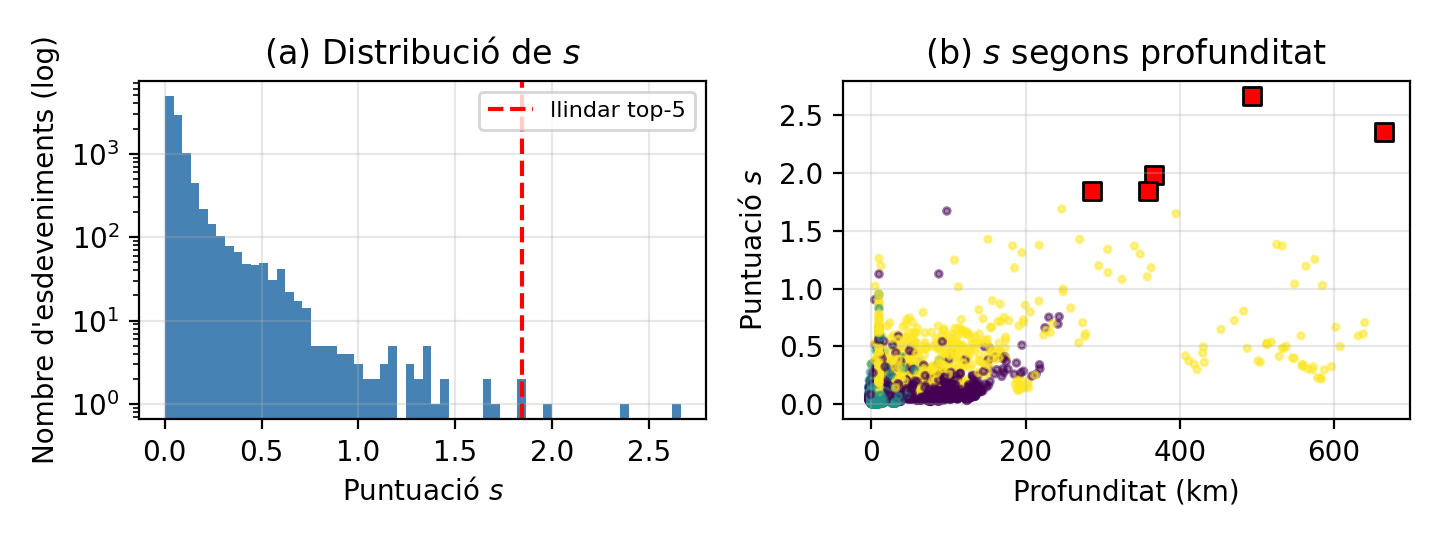
\includegraphics[width=0.78\textwidth]{fig_anom.png}
\caption{(a) Distribució de $s$ (escala log): cua molt llarga; mediana $0{,}047$, percentil 99 $=0{,}65$, màxim $2{,}67$. (b) $s$ segons la profunditat; quadrats vermells = top-5.}\label{fig:an}
\end{figure}
\textbf{Interpretació.} Les cinc anomalies són terratrèmols \textbf{profunds (286--665~km)} de zones de subducció amb sismicitat profunda coneguda \cite{frohlich} (mar d'Okhotsk, Vanuatu, mar Tirrè, Nova Zelanda, Bolívia). No destaquen per energia ($M\approx4$--$5$) sinó per \emph{raresa multivariant}: profunditat molt per sobre de la mediana del catàleg ($8{,}1$~km) i ubicació aïllada. El terratrèmol més gran ($M=7{,}7$, Panamà, 12,6~km) té $s=1{,}20$ i només és el \#23: el mètode detecta raresa, no gravetat. Cap anomalia és una voladura o explosió. Entre els 50 primers, 18 dels 58 esdeveniments del catàleg amb profunditat $>300$~km (mediana de profunditat del top-50: $217{,}6$~km).

\textbf{Sensibilitat a $k$ i contrast amb altres mètodes.}
\begin{table}[H]
\centering\footnotesize
\begin{tabular}{@{}lccc@{}}
\toprule
Comparació amb el top-5 base ($k=5$) & Coincidència top-5 & Coincidència top-50 & Spearman\\
\midrule
kNN, $k=3$ / $k=10$ / $k=20$ & 5/5 / 4/5 / 4/5 & --- & ---\\
Isolation Forest (200 arbres) & 0/5 & 10/50 & 0,61\\
LOF ($20$ veïns) & 0/5 & 6/50 & 0,40\\
\bottomrule
\end{tabular}
\caption{Robustesa de la llista d'anomalies.}\label{tab:rob}
\end{table}
La llista és molt estable respecte a $k$ (4--5 de 5 coincidències), però \textbf{no coincideix amb altres detectors}: Isolation Forest destaca esdeveniments profunds de la regió de Fiji ($519$--$640$~km, $M=4{,}8$--$5{,}9$) i LOF els de Panamà ($M=6{,}6$ i $7{,}7$) i alguns esdeveniments aïllats d'Austràlia, Nova Zelanda i Utah. La correlació de rangs és moderada ($0{,}61$ i $0{,}40$). No és una contradicció: cada mètode formalitza ``anomalia'' de manera diferent (aïllament, densitat relativa, distància als veïns); el kNN premia els esdeveniments \emph{individualment aïllats}, mentre que, probablement, una zona profunda amb molts esdeveniments (Fiji) els fa semblar veïns entre si i en redueix la puntuació. Per això convé donar la llista kNN com a ``candidats a revisió'' i no com a veritat.

\subsection{Eficiència}
Execució en l'entorn de prova (Python 3.12.3, scikit-learn 1.8.0, pandas 3.0.2, $n=10\,174$): \py{presentacio_MATIAS.py} triga $\approx2{,}2$~s en total (\py{KMeans} $\approx0{,}05$~s, kNN exacte $\approx0{,}06$~s), i \py{validacio_MATIAS.py} $\approx3{,}2$~s (inclou 7 valors de $K$, 5 llavors i la silueta). El cost del kNN exacte és $O(n^2)$ en el pitjor cas, però per a $n\sim10^4$ és negligible (O4 complert); per a milions d'esdeveniments caldria un índex d'arbre (\py{algorithm="kd_tree"}) o aproximació.

%------------------------------------------------------------
\section{Conclusions, limitacions i millores}\label{sec:lim}
\begin{table}[H]
\centering\footnotesize
\begin{tabular}{@{}cp{9.2cm}p{4.6cm}@{}}
\toprule
Obj. & Resultat & Estat\\
\midrule
O1 & $10\,174/10\,174$ files conservades & Complert\\
O2 & $K=3$: $5\,721/3\,414/1\,039$; silueta $0{,}402>0{,}3$ & Complert (grups geogràfics)\\
O3 & Top-5: terratrèmols profunds (286--665~km) de zones de subducció & Complert\\
O4 & ARI $=1$ per a 5 llavors; fases $<0{,}1$~s & Complert\\
O5 & $K=2$ té millor silueta; llista kNN estable en $k$ però diferent d'IF i LOF & Parcial: validació interna\\
\bottomrule
\end{tabular}
\caption{Compliment dels objectius.}\label{tab:obj}
\end{table}
\textbf{Conclusions.} (1) El pipeline és ràpid i reproduïble, i el clustering és perfectament estable amb \py{k-means++} i 10 inicialitzacions. (2) Els tres clústers separen \emph{xarxes i regions}, no tipus de sisme: el clúster global és gran per cobertura del catàleg; només sense variables geogràfiques apareix un grup físic de terratrèmols profunds. (3) El detector kNN troba terratrèmols profunds i aïllats, geofísicament coherents, però la llista depèn del mètode, de manera que s'ha d'interpretar com a candidats a revisió.

\textbf{Limitacions.} (i) Latitud i longitud en graus euclidians distorsionen les distàncies reals i la longitud és circular. (ii) Barreja d'escales de magnitud i de 236 esdeveniments no sísmics. (iii) $K$ fix; la silueta prefereix $K=2$. (iv) Catàleg d'un sol mes i sense veritat de referència: la validació és interna. (v) Les proves verifiquen la correcció del codi i la reproducció de les xifres, però no la validesa científica de les conclusions (que depèn de la validació de la Secció~\ref{sec:res}).

\textbf{Millores concretes.} (1) Filtrar \py{type == "earthquake"}; (2) usar coordenades cartesianes 3D (o distància haversine) per resoldre la circularitat; (3) clustering només sobre magnitud i profunditat, o amb pesos per variable; (4) combinar kNN, LOF i Isolation Forest (consens de rangs); (5) afegir una interfície de línia d'ordres (\py{argparse}) per canviar $K$, $k$ i el fitxer sense editar el codi i mesurar la cobertura de les proves; (6) ampliar a diversos mesos per provar la robustesa temporal.

%------------------------------------------------------------
\section{Reproducibilitat}
Entorn: Python 3.12.3, scikit-learn 1.8.0, pandas 3.0.2, matplotlib 3.10.8, NumPy 2.4.4, SciPy; versions fixades al \py{requirements.txt}. Instruccions al \py{README}. Fitxers: \py{presentacio_MATIAS.py} (Taules~\ref{tab:cl} i~\ref{tab:an}, Fig.~\ref{fig:cl}a), \py{validacio_MATIAS.py} (Taules~\ref{tab:k} i~\ref{tab:rob}, estabilitat, Figs.~\ref{fig:cl}b, \ref{fig:k} i~\ref{fig:an}, i les proves) i \py{earthquakes.csv} (dades d'exemple, mateix directori). Ordres: \py{python presentacio_MATIAS.py} i \py{python validacio_MATIAS.py} (executa primer les proves); només les proves: \py{python -m unittest -v validacio_MATIAS}. Totes les llavors són fixes (42), per tant la sortida és determinista amb les mateixes dades i versions.

\begin{thebibliography}{99}\footnotesize
\setlength{\itemsep}{0pt}
\bibitem{usgs} U.S.\ Geological Survey. \emph{ANSS Comprehensive Earthquake Catalog (ComCat)}. \url{https://earthquake.usgs.gov/earthquakes/search/}
\bibitem{gr} Gutenberg, B., Richter, C.\ F. (1944). Frequency of earthquakes in California. \emph{Bull.\ Seismol.\ Soc.\ Am.}, 34(4), 185--188.
\bibitem{lloyd} Lloyd, S.\ P. (1982). Least squares quantization in PCM. \emph{IEEE Trans.\ Inf.\ Theory}, 28(2), 129--137.
\bibitem{macqueen} MacQueen, J. (1967). Some methods for classification and analysis of multivariate observations. \emph{Proc.\ 5th Berkeley Symp.}, 1, 281--297.
\bibitem{kmpp} Arthur, D., Vassilvitskii, S. (2007). k-means++: the advantages of careful seeding. \emph{Proc.\ SODA}, 1027--1035.
\bibitem{ramaswamy} Ramaswamy, S., Rastogi, R., Shim, K. (2000). Efficient algorithms for mining outliers from large data sets. \emph{Proc.\ ACM SIGMOD}, 427--438.
\bibitem{lof} Breunig, M.\ M., Kriegel, H.-P., Ng, R.\ T., Sander, J. (2000). LOF: identifying density-based local outliers. \emph{Proc.\ ACM SIGMOD}, 93--104.
\bibitem{iforest} Liu, F.\ T., Ting, K.\ M., Zhou, Z.-H. (2008). Isolation forest. \emph{Proc.\ IEEE ICDM}, 413--422.
\bibitem{chandola} Chandola, V., Banerjee, A., Kumar, V. (2009). Anomaly detection: a survey. \emph{ACM Comput.\ Surv.}, 41(3), 15.
\bibitem{rousseeuw} Rousseeuw, P.\ J. (1987). Silhouettes: a graphical aid to the interpretation and validation of cluster analysis. \emph{J.\ Comput.\ Appl.\ Math.}, 20, 53--65.
\bibitem{kaufman} Kaufman, L., Rousseeuw, P.\ J. (1990). \emph{Finding Groups in Data}. Wiley.
\bibitem{db} Davies, D.\ L., Bouldin, D.\ W. (1979). A cluster separation measure. \emph{IEEE Trans.\ Pattern Anal.\ Mach.\ Intell.}, 1(2), 224--227.
\bibitem{hubert} Hubert, L., Arabie, P. (1985). Comparing partitions. \emph{J.\ Classification}, 2(1), 193--218.
\bibitem{frohlich} Frohlich, C. (2006). \emph{Deep Earthquakes}. Cambridge University Press.
\bibitem{sklearn} Pedregosa, F.\ et al.\ (2011). Scikit-learn: machine learning in Python. \emph{J.\ Mach.\ Learn.\ Res.}, 12, 2825--2830.
\bibitem{pandas} McKinney, W. (2010). Data structures for statistical computing in Python. \emph{Proc.\ 9th Python in Science Conf.}, 56--61.
\bibitem{mpl} Hunter, J.\ D. (2007). Matplotlib: a 2D graphics environment. \emph{Comput.\ Sci.\ Eng.}, 9(3), 90--95.
\end{thebibliography}
\end{document}
